\documentclass[12pt,a4paper,twoside]{report}
% -------------------------------------------------------------------- %
% Pacotes

\usepackage[utf8]{inputenc}
\usepackage[T1]{fontenc}
\usepackage[brazil]{babel}
\usepackage[fixlanguage]{babelbib}
\usepackage[pdftex]{graphicx}      % usamos arquivos pdf/png como figuras
\usepackage{setspace}              % espaçamento flexvel
\usepackage{indentfirst}           % indentação do primeiro parágrafo
\usepackage{makeidx}               % índice remissivo
\usepackage[nottoc]{tocbibind}     % acrescentamos a bibliografia/indice/conteudo no Table of Contents
\usepackage{courier}               % usa o Adobe Courier no lugar de Computer Modern Typewriter
\usepackage{type1cm}               % fontes realmente escaláveis
\usepackage{titletoc}
\usepackage{ucs}
\usepackage[font=small,format=plain,labelfont=bf,up,textfont=it,up]{caption}
\usepackage[usenames,svgnames,dvipsnames]{xcolor}
\usepackage[a4paper,top=2.54cm,bottom=2.0cm,left=2.0cm,right=2.54cm]{geometry} % margens
\usepackage{amsmath} 

\usepackage[pdftex,plainpages=false,pdfpagelabels,pagebackref,colorlinks=true,citecolor=DarkGreen,
linkcolor=NavyBlue,urlcolor=DarkRed,filecolor=green,bookmarksopen=true]{hyperref} % links coloridos
\usepackage[all]{hypcap}                % soluciona o problema com o hyperref e capítulos
\usepackage[square,sort,nonamebreak,comma]{natbib}  % citação bibliográfica alpha
\fontsize{60}{62}\usefont{OT1}{cmr}{m}{n}{\selectfont}
\usepackage{upquote}                    % formata apóstrofes '
\usepackage{textcomp}

% Para formatar corretamente as URLs
\usepackage{url}
% -------------------------------------------------------------------- %
% Cabeçalhos similares ao TAOCP de Donald E. Knuth
\usepackage{fancyhdr}
\pagestyle{fancy}
\fancyhf{}
\renewcommand{\chaptermark}[1]{\markboth{\MakeUppercase{#1}}{}}
\renewcommand{\sectionmark}[1]{\markright{\MakeUppercase{#1}}{}}
\renewcommand{\headrulewidth}{0pt}

% -------------------------------------------------------------------- %
\graphicspath{{./imagens/}}        % caminho das figuras
\frenchspacing                     % arruma o espaço: id est (i.e.) e exempli gratia (e.g.)
\urlstyle{same}                    % URL com o mesmo estilo do texto e no mono-spaced
\makeindex                         % para o índice remissivo
\raggedbottom                      % para no permitir espaços extras no texto
\fontsize{60}{62}\usefont{OT1}{cmr}{m}{n}{\selectfont}
\cleardoublepage
\normalsize

% -------------------------------------------------------------------- %
% Cores para formatação de código
\usepackage{color}
\definecolor{vermelho}{rgb}{0.6,0,0} % para strings
\definecolor{verde}{rgb}{0.25,0.5,0.35} % para comentários
\definecolor{roxo}{rgb}{0.5,0,0.35} % para palavras-chaves
\definecolor{azul}{rgb}{0.25,0.35,0.75} % para strings
\definecolor{cinza-claro}{gray}{0.95}
% -------------------------------------------------------------------- %
% Opções de listagem usados para o código fonte
% Ref: http://en.wikibooks.org/wiki/LaTeX/Packages/Listings



\usepackage{listings}           % para formatar código-fonte (ex. em Java)


\lstset{ %
language=Python,                      % seleciona a linguagem do código
basicstyle=\footnotesize\ttfamily,    % o tamanho da fonte usado no código
commentstyle=\color{verde}\bfseries,  % formatação de comentários
stringstyle=\color{azul},             % formatação de strings
upquote=true,
numbers=left,                   % onde colocar os números de linha
numberstyle=\tiny,  % o tamanho da fonte usada para a numeração das linhas
stepnumber=1,                   % o intervalo entre dois números de linhas. Se for 1, numera cada uma.
numbersep=5pt,                  % how far the line-numbers are from the code
showspaces=false,               % show spaces adding particular underscores
showstringspaces=false,         % underline spaces within strings
showtabs=false,                 % show tabs within strings adding particular underscores
keywordstyle=\color{roxo}\bfseries,
keywordstyle=[1]\color{roxo}\bfseries,
keywordstyle=[2]\color{verde}\bfseries,
frame=b,                   % adds a frame around the code
framerule=0.6pt,
tabsize=2,                      % sets default tabsize to 2 spaces
captionpos=t,                   % sets the caption-position to top
breaklines=true,                % sets automatic line breaking
breakatwhitespace=false,        % sets if automatic breaks should only happen at whitespace
escapeinside={\%*}{*)},         % if you want to add a comment within your code
backgroundcolor=\color[rgb]{1.0,1.0,1.0}, % choose the background color.
rulecolor=\color[rgb]{0.8,0.8,0.8},
extendedchars=true,
xleftmargin=10pt,
xrightmargin=10pt,
framexleftmargin=10pt,
framexrightmargin=10pt,
literate={â}{{\^{a}}}1  % para formatar corretamente os acentos do Português ao usar utf8
    {ê}{{\^{e}}}1
    {ô}{{\^{o}}}1  
    {Â}{{\^{A}}}1
    {Ê}{{\^{E}}}1
    {Ô}{{\^{O}}}1
    {á}{{\'{a}}}1
    {é}{{\'{e}}}1
    {í}{{\'{i}}}1
    {ó}{{\'{o}}}1
    {ú}{{\'{u}}}1
    {Á}{{\'{A}}}1
    {É}{{\'{E}}}1
    {Í}{{\'{I}}}1
    {Ó}{{\'{O}}}1
    {Ú}{{\'{U}}}1
    {à}{{\`{a}}}1
    {À}{{\`{A}}}1
    {ã}{{\~{a}}}1
    {õ}{{\~{o}}}1
    {Ã}{{\~{A}}}1
    {Õ}{{\~{O}}}1
    {ç}{{\c{c}}}1
    {Ç}{{\c{C}}}1
    {ü}{{\"u}}1
    {Ü}{{\"U}}1
}

\renewcommand{\lstlistingname}{Listagem}
\renewcommand{\lstlistlistingname}{Lista de Listagens}

% Definição de novos estilos
\lstdefinestyle{Bash}
    {language=bash,frame=single,numbers=none,basicstyle=\footnotesize\ttfamily,
     morekeywords={cp,mkdir,sudo,tar}}

% Definição de novos ambientes
\lstnewenvironment{terminal}
  {\lstset{style=Bash}}
  {}

\lstnewenvironment{python}
  {\lstset{basicstyle=\scriptsize\ttfamily,
           frame=single,
           frameround=tttt,
           framerule=2pt,
           numbers=none,
           rulecolor=\color{Salmon}}}
  {}

\lstnewenvironment{ide}
  {\lstset{frame=single,
            frameround=tttt,
            numbers=none,
            basicstyle=\ttfamily,
            framerule=2pt,
            rulecolor=\color{CadetBlue}}}
  {}

\lstnewenvironment{latex}
   {\lstset{language=[LaTex]TeX,
            basicstyle=\scriptsize\ttfamily,
            frame=none,
            numbers=none}}
   {}


% Formata o caption da listagem
% \DeclareCaptionFont{blue}{\color{blue}} 

% \captionsetup[lstlisting]{singlelinecheck=false, labelfont={blue}, textfont={blue}}
\usepackage{caption}
\DeclareCaptionFont{white}{\color{white}}
\DeclareCaptionFormat{listing}{\colorbox[cmyk]{0.43, 0.35, 0.35,0.01}{\parbox{\textwidth}{\hspace{15pt}#1#2#3}}}
\captionsetup[lstlisting]{format=listing,labelfont=white,textfont=white, singlelinecheck=false, margin=0pt, font={bf,footnotesize}}

\newcommand{\ListingsPath}{./codigos}
% Inclui o nome do arquivo como Caption 
\newcommand{\filelisting}[2][]{%
    \lstinputlisting[caption={\texttt{\detokenize{#2}}},#1]{\ListingsPath/#2}%
}

% ---------------------------------------------------------------------------- %

% ---------------------------------------------------------------------------- %

\title{Análise de Complexidade de Tempo do Método Bubble Sort}
\date{}
\author{Eduardo Costa de Paiva \\
\texttt{\small \url{eduardocspv@gmail.com}}\\
Frederico Franco Calhau \\
\texttt{\small \url{fredericoffc@gmail.com}}\\
Gabriel Augusto Marson \\
\texttt{\small \url{gabrielmarson@live.com}}\\
\vspace{1cm} \\
Faculdade de Computação \\
Universidade Federal de Uberlândia
}
\date{\today}

\begin{document}
  \maketitle
% -------------------------------------------------------------------- %
% Listas de figuras, tabelas e códigos criadas automaticamente
\listoffigures            
\listoftables            
\lstlistoflistings
% -------------------------------------------------------------------- %

% -------------------------------------------------------------------- %
% Sumário
\tableofcontents    

% Capítulos do trabalho

% cabeçalho para as páginas de todos os capítulos
\fancyhead[RE,LO]{\thesection}

%\singlespacing              % espaçamento simples
\setlength{\parskip}{0.15in} % espaçamento entre paragráfos

\chapter{Introdução}
Este documento foi feito com o intuito de exibir uma análise do algoritmo Bubble Sort 
com relação a tempo. Além disso, será feita uma comparação da curva de tempo do que se espera do
algoritmo, ou seja, $O(n^2)$ com o caso prático. 

\section{Diretório}

Dada a seguinte organização das pastas, utilizamos o arquivo testdriver.py,  executando, uma função conveniente por vez. Para mais informações vá até ao apêndice.

OBS.: É necessário instalar o programa tree pelo terminal. Isso pode ser feito da seguinte maneira.

\begin{terminal}
> sudo apt-get install tree
\end{terminal}

A seguir é mostrada a organização das pastas sendo que os diretórios significativas para o projeto são Codigos e Relatorio além do raíz:
\begin{terminal}
tree --charset=ASCII
.
|-- Codigos
|   |-- Bubble
|   |   |-- BubbleSort.py
|   |   `-- __pycache__
|   |       |-- BubbleSort.cpython-34.pyc
|   |       `-- testeBubble.cpython-34.pyc
|   `-- README.md
|-- memoria.py
|-- monitor.py
|-- Other
|   |-- expfit0.py
|   |-- expfit.py
|   |-- leialprof.py
|   |-- leitura1.py
|   |-- leitura2.py
|   |-- leitura.py
|   `-- logfit.py
|-- Plot
|   |-- plot1.py
|   |-- plot2.py
|   |-- plot3.py
|   `-- plot_tempo.py
|-- __pycache__
|   |-- monitor.cpython-34.pyc
|   `-- tempo.cpython-34.pyc
|-- relatorio
|   |-- imagens
|   |   |-- Bubble
|   |   |   |-- bubble_plot_1.png
|   |   |   `-- bubble_plot_3.png
|   |   `-- Merge
|   |-- Relatorio_Bubble
|   |   |-- RelatorioBubble.aux
|   |   |-- RelatorioBubble.idx
|   |   |-- RelatorioBubble.lof
|   |   |-- RelatorioBubble.log
|   |   |-- RelatorioBubble.lol
|   |   |-- RelatorioBubble.lot
|   |   |-- RelatorioBubble.out
|   |   |-- RelatorioBubble.tex
|   |   `-- RelatorioBubble.toc
|   |-- Relatorio_Merge
|   `-- Resultados
|       |-- Bubble
|       |   `-- tBolha.dat
|       `-- Merge
|-- tempo.py
|-- testdriver.py
|-- testeGeneric.py
`-- testeGeneric.py.lprof

15 directories, 35 files

\end{terminal}

\section{Códigos de programas}
Seguem os códigos utilizados na análise de tempo do algoritmo Bubble Sort.
\begin{enumerate}

\item BubbleSort.py:
Disponível na Listagem~\ref{arq:BubbleSort}.
\lstinputlisting[caption={BubbleSort.py \label{arq:BubbleSort}}]{../../Codigos/Bubble/BubbleSort.py}

\item testeGeneric.py
Disponível na Listagem ~\ref{arq:testeGeneric}
\lstinputlisting[caption={testeGeneric.py \label{arq:testeGeneric}}]{../../testeGeneric.py}

\item monitor.py
Disponível na Listagem~\ref{arq:monitor}
\lstinputlisting[caption={monitor.py \label{arq:monitor}}]{../../monitor.py}


\item testdriver.py
 Referenciado no apêndice~\ref{ap:testdriver}.
\end{enumerate}


\chapter{Gráficos}

Seguem os Gráficos utilizadas no processo de análise do método Bubble Sort:
\begin{enumerate}

	\item Para um vetor aleatório
	\begin{enumerate}
		\item Complexidade de custo do método da bolha disponível na lista de imagens ~\ref{fig:BubblePlot1A}.
		\begin{figure}[!h]
			\centering
			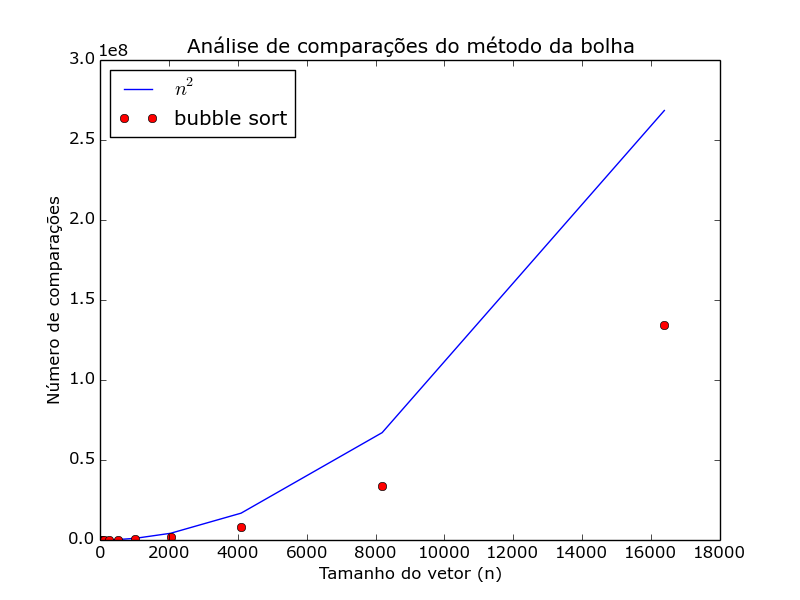
\includegraphics[scale=0.6]{../imagens/Bubble/bubble_plot_1_aleatorio.png}
			\caption{Complexidade de custo do método da bolha (Vetor Aleatório) \label{fig:BubblePlot1A}}
		\end{figure}
		
		
		\item Complexidade de tempo do método da bolha disponível na lista de imagens ~\ref{fig:BubblePlot2A}.
		\begin{figure}[!h]
			\centering
			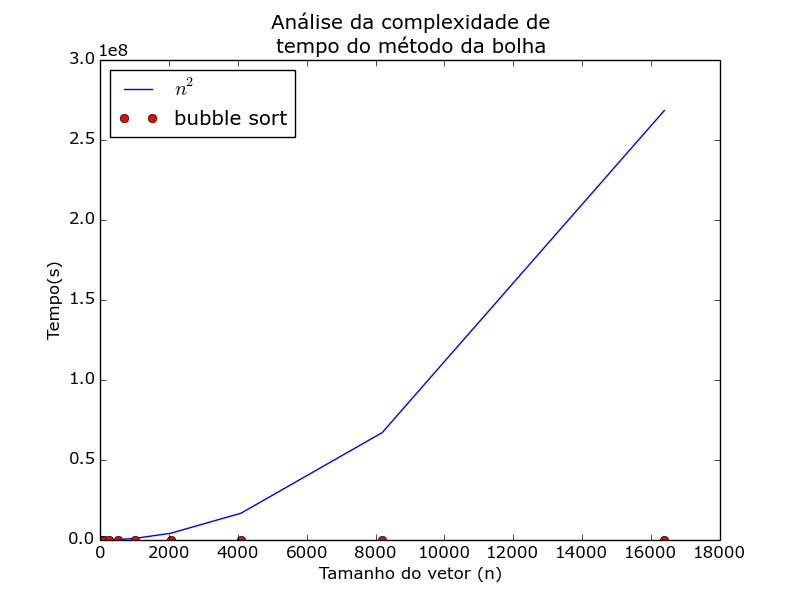
\includegraphics[scale=0.6]{../imagens/Bubble/bubble_plot_2_aleatorio.png}
			\caption{Complexidade de tempo do método da bolha (Vetor Aleatório)\label{fig:BubblePlot2A}}
		\end{figure}
		
		
		\item Complexidade de tempo do método da bolha com mínimos quadrados disponível na lista de imagens ~\ref{fig:BubblePlot3A}.
		\begin{figure}[!h]
			\centering
			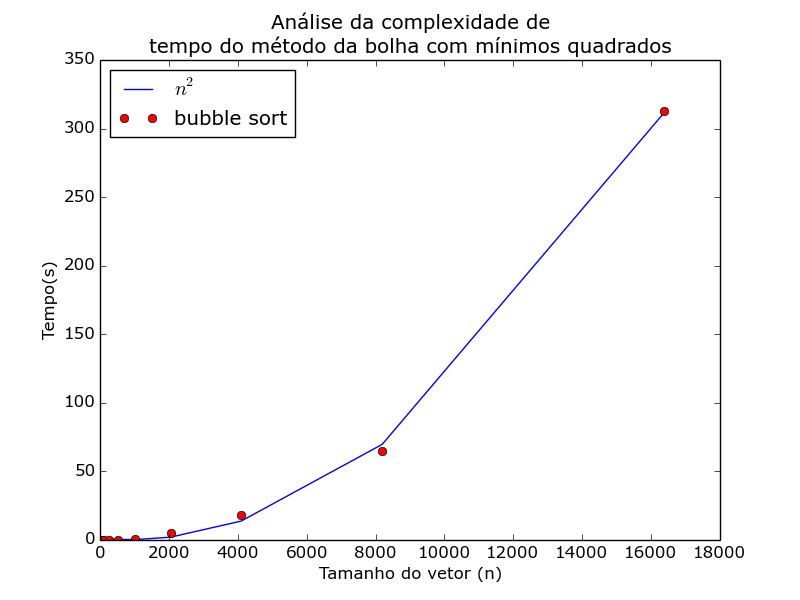
\includegraphics[scale=0.6]{../imagens/Bubble/bubble_plot_3_aleatorio.png}
			\caption{Complexidade de tempo do método da bolha com mínimos quadrados (Vetor Aleatório) \label{fig:BubblePlot3A}}
		\end{figure}
	
	\end{enumerate}
	
	\item Para um vetor ordenado crescente
		\begin{enumerate}
			\item Complexidade de custo do método da bolha disponível na lista de imagens ~\ref{fig:BubblePlot1OC}.
			\begin{figure}[!h]
				\centering
				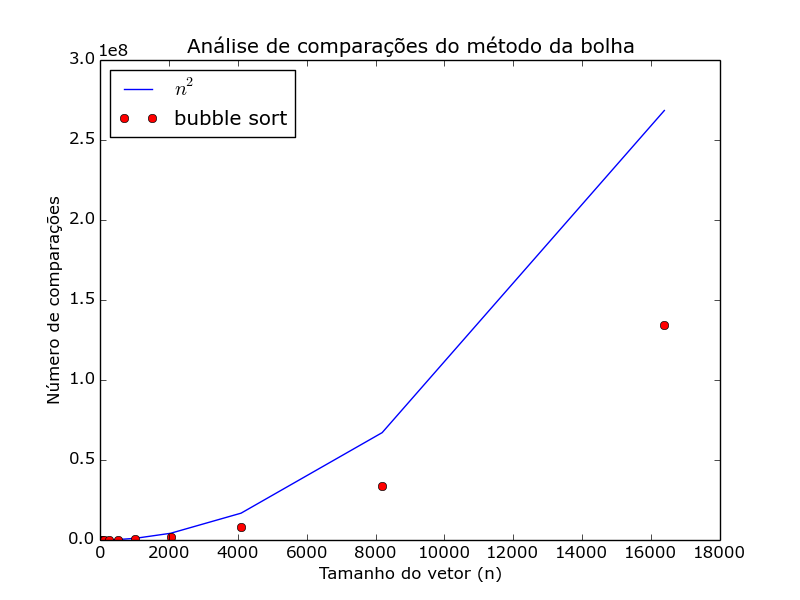
\includegraphics[scale=0.6]{../imagens/Bubble/bubble_plot_1_ordenado_crescente.png}
				\caption{Complexidade de custo do método da bolha (Vetor Ordenado Crescente)\label{fig:BubblePlot1OC}}
			\end{figure}
			
			
			\item Complexidade de tempo do método da bolha disponível na lista de imagens ~\ref{fig:BubblePlot2OC}.
			\begin{figure}[!h]
				\centering
				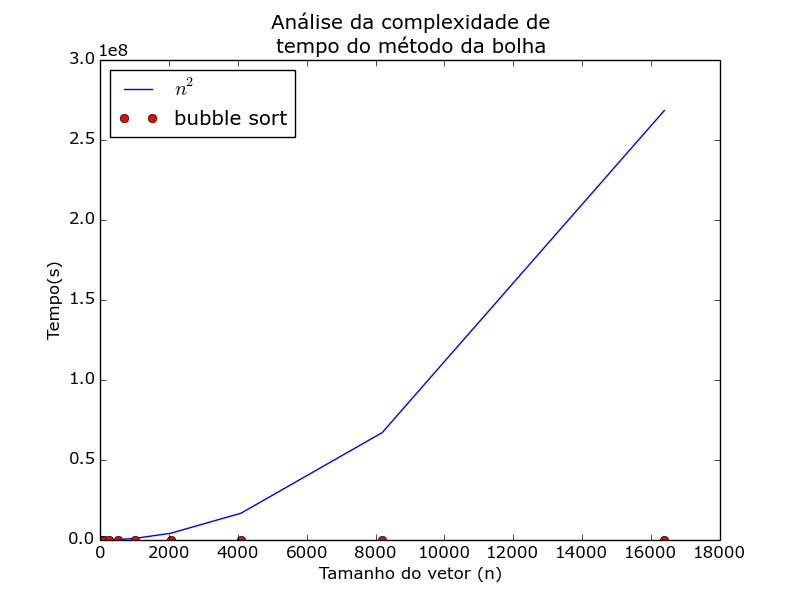
\includegraphics[scale=0.6]{../imagens/Bubble/bubble_plot_2_ordenado_crescente.png}
				\caption{Complexidade de tempo do método da bolha (Vetor Ordenado Crescente) \label{fig:BubblePlot2OC}}
			\end{figure}
			
			
			\item Complexidade de tempo do método da bolha com mínimos quadrados disponível na lista de imagens ~\ref{fig:BubblePlot3OC}.
			\begin{figure}[!h]
				\centering
				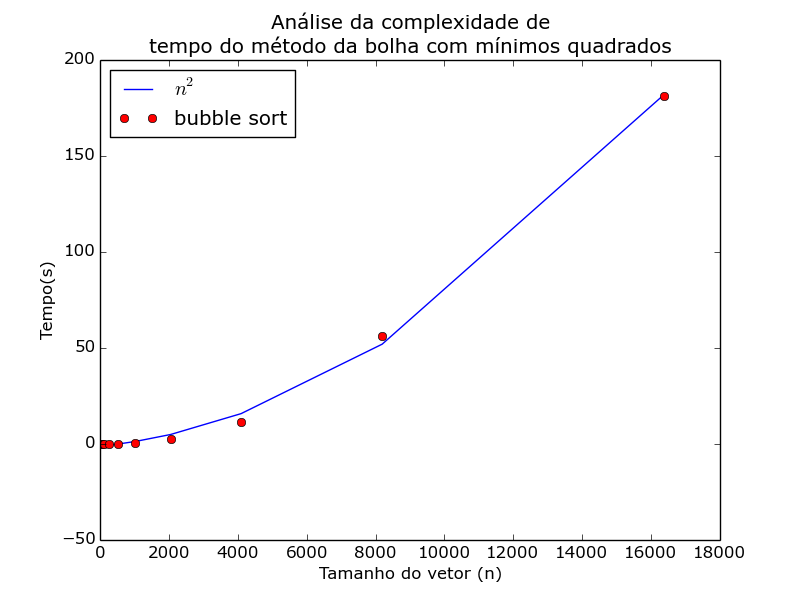
\includegraphics[scale=0.6]{../imagens/Bubble/bubble_plot_3_ordenado_crescente.png}
				\caption{Complexidade de tempo do método da bolha com mínimos quadrados (Vetor Ordenado Crescente) \label{fig:BubblePlot3OC}}
			\end{figure}
		
		\end{enumerate}
	
		
		
		\item Para um vetor ordenado decrescente
				\begin{enumerate}
					\item Complexidade de custo do método da bolha disponível na lista de imagens ~\ref{fig:BubblePlot1OD}.
					\begin{figure}[!h]
						\centering
						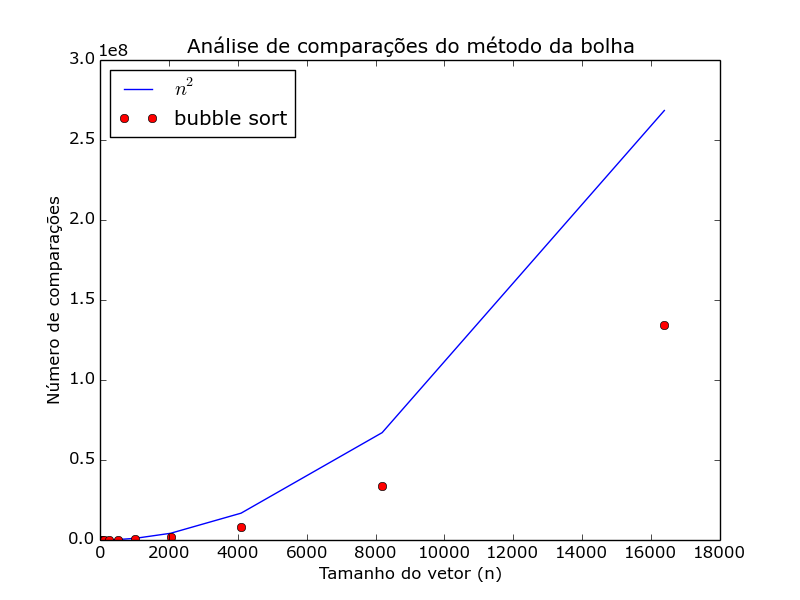
\includegraphics[scale=0.6]{../imagens/Bubble/bubble_plot_1_ordenado_decrescente.png}
						\caption{Complexidade de custo do método da bolha (Vetor Ordenado Decrescente) \label{fig:BubblePlot1OD}}
					\end{figure}
					
					
					\item Complexidade de tempo do método da bolha disponível na lista de imagens ~\ref{fig:BubblePlot2OD}.
					\begin{figure}[!h]
						\centering
						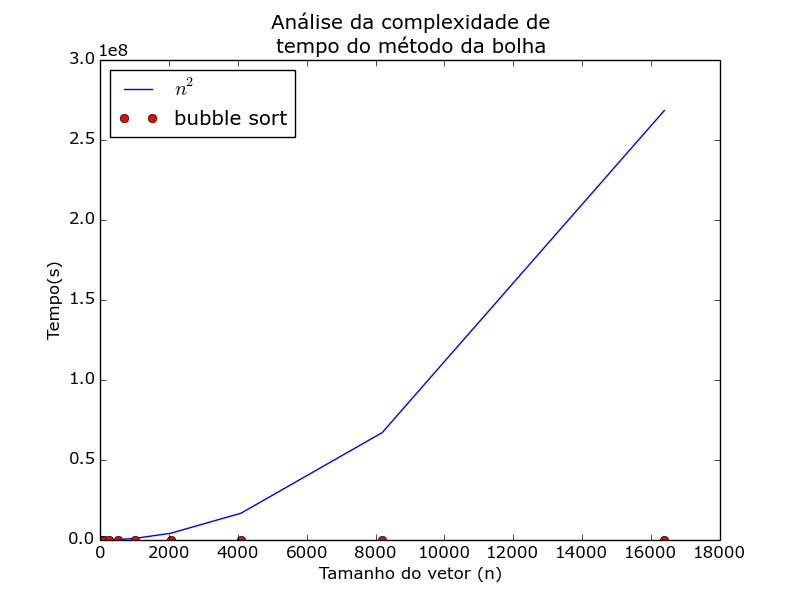
\includegraphics[scale=0.6]{../imagens/Bubble/bubble_plot_2_ordenado_decrescente.png}
						\caption{Complexidade de tempo do método da bolha (Vetor Ordenado Decrescente) \label{fig:BubblePlot2OD}}
					\end{figure}
					
					
					\item Complexidade de tempo do método da bolha com mínimos quadrados disponível na lista de imagens  ~\ref{fig:BubblePlot3OD}.
					\begin{figure}[!h]
						\centering
						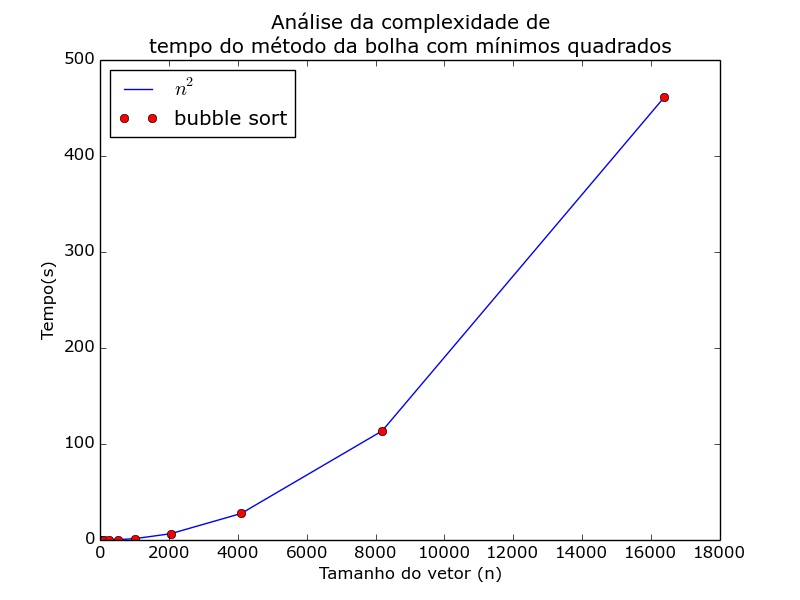
\includegraphics[scale=0.6]{../imagens/Bubble/bubble_plot_3_ordenado_decrescente.png}
						\caption{Complexidade de tempo do método da bolha com mínimos quadrados (Vetor Ordenado Decrescente) \label{fig:BubblePlot3OD}}
					\end{figure}
				
				\end{enumerate}
				
				
			\item Para um vetor parcialmente ordenado crescente
							\begin{enumerate}
								\item Complexidade de custo do método da bolha disponível na lista de imagens ~\ref{fig:BubblePlot1POC}.
								\begin{figure}[!h]
									\centering
									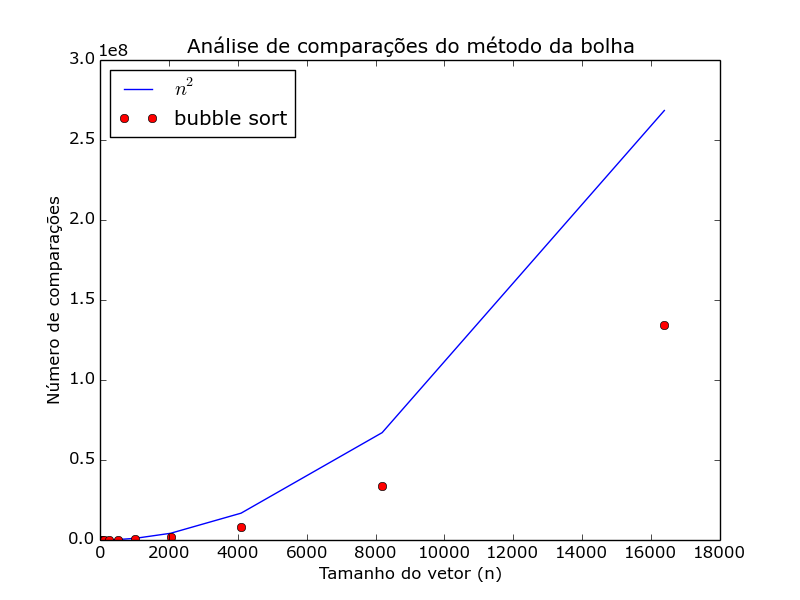
\includegraphics[scale=0.6]{../imagens/Bubble/bubble_plot_1_parcialmente_ordenado_crescente.png}
									\caption{Complexidade de custo do método da bolha (Vetor Parcialmente Ordenado Crescente) \label{fig:BubblePlot1POC}}
								\end{figure}
								
								
								\item Complexidade de tempo do método da bolha disponível na lista de imagens ~\ref{fig:BubblePlot2POC}.
								\begin{figure}[!h]
									\centering
									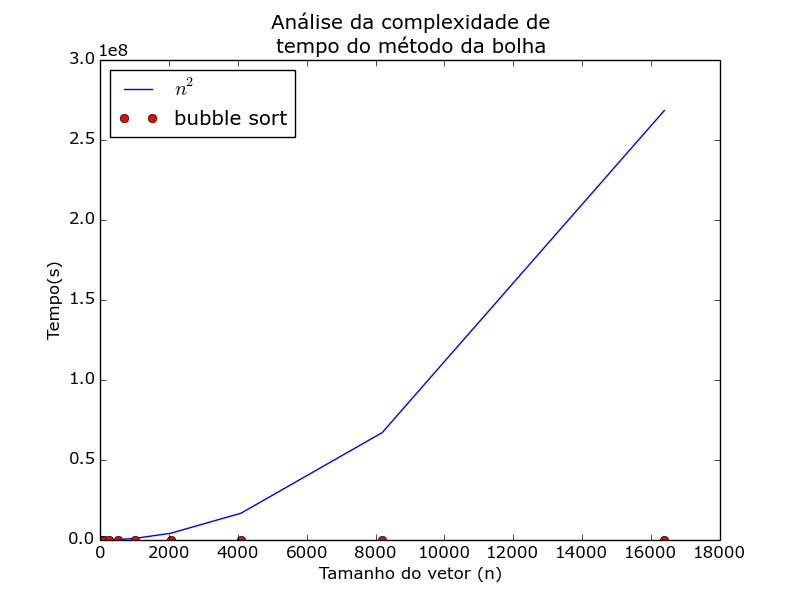
\includegraphics[scale=0.6]{../imagens/Bubble/bubble_plot_2_parcialmente_ordenado_crescente.png}
									\caption{Complexidade de tempo do método da bolha (Vetor Parcialmente Ordenado Crescente) \label{fig:BubblePlot2POC}}
								\end{figure}
								
								
								\item Complexidade de tempo do método da bolha com mínimos quadrados disponível na lista de imagens  ~\ref{fig:BubblePlot3POC}.
								\begin{figure}[!h]
									\centering
									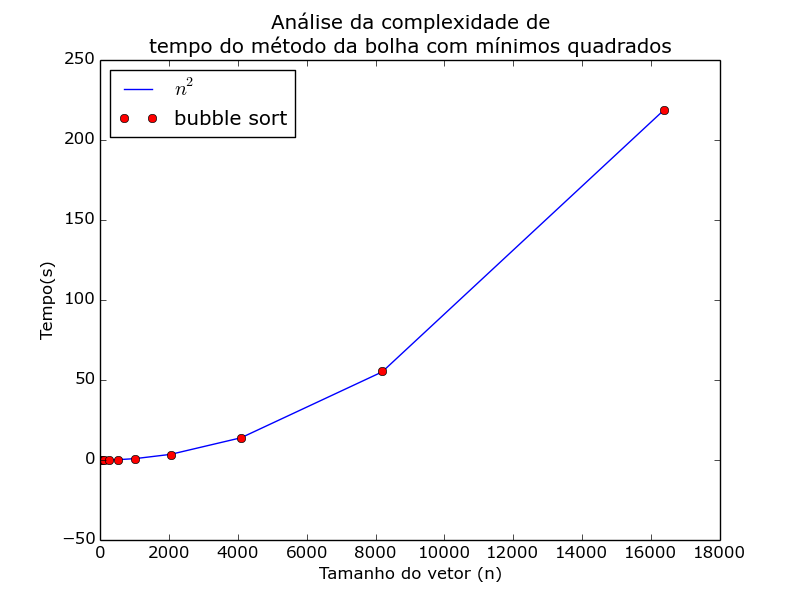
\includegraphics[scale=0.6]{../imagens/Bubble/bubble_plot_3_parcialmente_ordenado_crescente.png}
									\caption{Complexidade de tempo do método da bolha com mínimos quadrados (Vetor Parcialmente Ordenado Crescente) \label{fig:BubblePlot3POC}}
								\end{figure}
							
							\end{enumerate}
			
			
			\item Para um vetor parcialmente ordenado decrescente
										\begin{enumerate}
											\item Complexidade de custo do método da bolha disponível na lista de imagens ~\ref{fig:BubblePlot1POD}.
											\begin{figure}[!h]
												\centering
												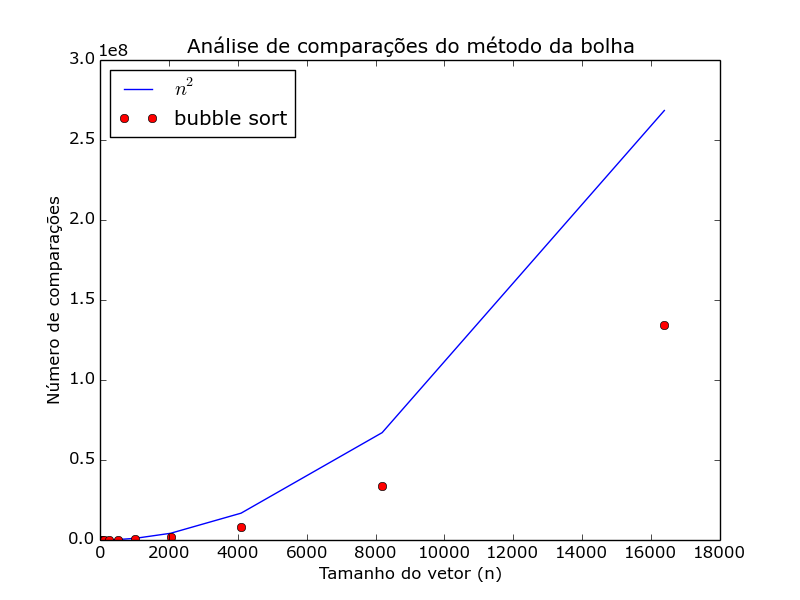
\includegraphics[scale=0.6]{../imagens/Bubble/bubble_plot_1_parcialmente_ordenado_decrescente.png}
												\caption{Complexidade de custo do método da bolha (Vetor Parcialmente Ordenado Decrescente) \label{fig:BubblePlot1POD}}
											\end{figure}
											
											
											\item Complexidade de tempo do método da bolha disponível na lista de imagens ~\ref{fig:BubblePlot2POD}.
											\begin{figure}[!h]
												\centering
												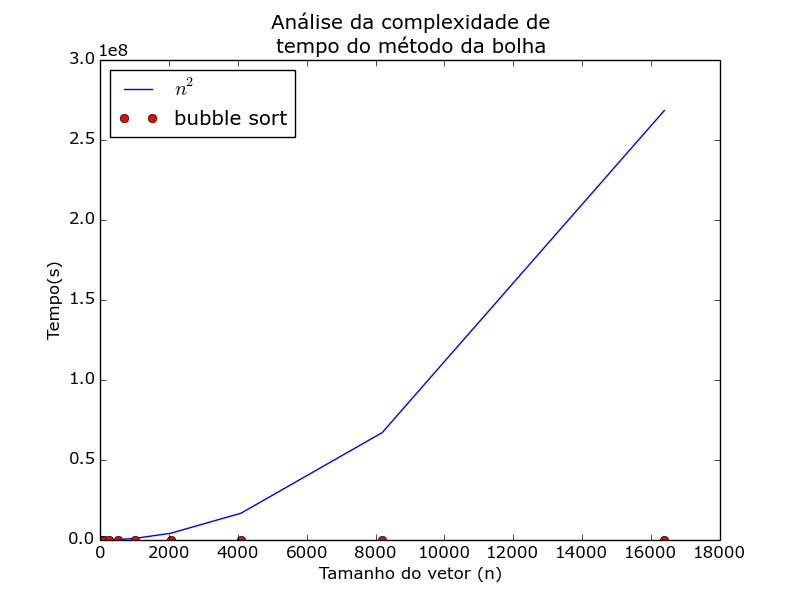
\includegraphics[scale=0.6]{../imagens/Bubble/bubble_plot_2_parcialmente_ordenado_decrescente.png}
												\caption{Complexidade de tempo do método da bolha (Vetor Parcialmente Ordenado Decrescente) \label{fig:BubblePlot2POD}}
											\end{figure}
											
											
											\item Complexidade de tempo do método da bolha com mínimos quadrados disponível na lista de imagens  ~\ref{fig:BubblePlot3POD}.
											\begin{figure}[!h]
												\centering
												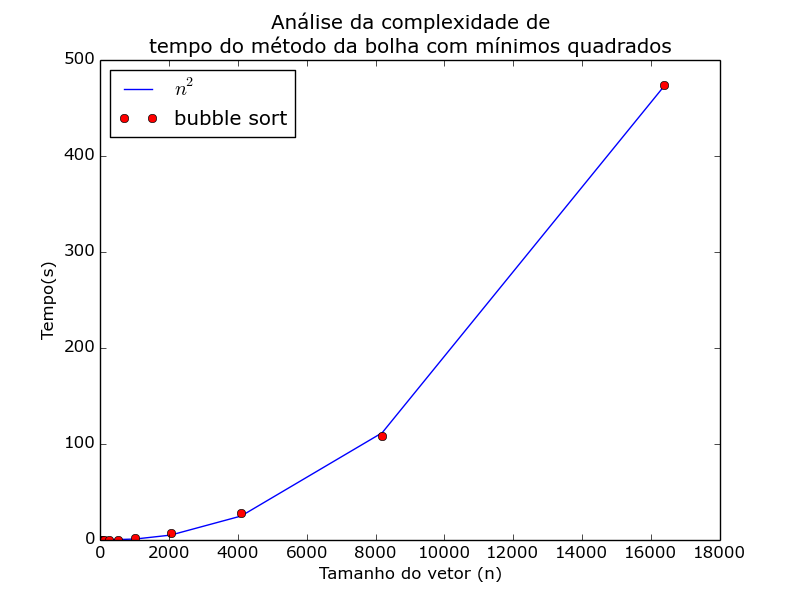
\includegraphics[scale=0.6]{../imagens/Bubble/bubble_plot_3_parcialmente_ordenado_decrescente.png}
												\caption{Complexidade de tempo do método da bolha com mínimos quadrados (Vetor Parcialmente Ordenado Decrescente) \label{fig:BubblePlot3POD}}
											\end{figure}
										
										\end{enumerate}
			
	
\end{enumerate}

\chapter{Tabelas}

Seguem as tabelas utilizadas para a análise do método Bubble Sort.

\begin{table}[h]
  \centering
  \caption{Vetor Aleatorio \label{tab:aleatorio}}
  \begin{tabular}{ccc} \\\hline
  \textbf{Tamanho do Vetor} & \textbf{Comparações} & \textbf{Tempo(s)} \\\hline
  32                        & 496                  & 0.000756          \\\hline
  64                        & 2016                 & 0.003263          \\\hline
  128                       & 8128                 & 0.012834          \\\hline
  256                       & 32640                & 0.050149          \\\hline
  512                       & 130816               & 0.200732          \\\hline
  1024                      & 523776               & 0.882822          \\\hline
  2048                      & 2096128              & 4.874270          \\\hline
  4096                      & 8386560              & 18.039000         \\\hline
  8192                      & 33550336             & 65.256400         \\\hline
  16384                     & 134209536            & 312.534000       \\\hline
  \end{tabular}
\end{table}


\begin{table}[h]
  \centering
  \caption{Vetor Ordenado Crescente \label{tab:oc}}
  \begin{tabular}{ccc} \\\hline
  \textbf{Tamanho do Vetor} & \textbf{Comparações} & \textbf{Tempo(s)} \\\hline
  32                        & 496                  & 0.000457          \\\hline
  64                        & 2016                 & 0.001817          \\\hline
  128                       & 8128                 & 0.007373          \\\hline
  256                       & 32640                & 0.028836          \\\hline
  512                       & 130816               & 0.114824          \\\hline
  1024                      & 523776               & 0.513465          \\\hline
  2048                      & 2096128              & 2.845550          \\\hline
  4096                      & 8386560              & 11.410900         \\\hline
  8192                      & 33550336             & 56.293100         \\\hline
  16384                     & 134209536            & 181.343000       \\\hline
  \end{tabular}
\end{table}


\begin{table}[h]
  \centering
  \caption{Vetor Ordenado Decrescente \label{tab:od}}
  \begin{tabular}{ccc} \\\hline
  \textbf{Tamanho do Vetor} & \textbf{Comparações} & \textbf{Tempo(s)} \\\hline
  32                        & 496                  & 0.001207          \\\hline
  64                        & 2016                 & 0.004553          \\\hline
  128                       & 8128                 & 0.018195          \\\hline
  256                       & 32640                & 0.073946          \\\hline
  512                       & 130816               & 0.299655          \\\hline
  1024                      & 523776               & 1.427660          \\\hline
  2048                      & 2096128              & 6.381420          \\\hline
  4096                      & 8386560              & 28.260700         \\\hline
  8192                      & 33550336             & 113.214000        \\\hline
  16384                     & 134209536            & 461.349000        \\\hline
  \end{tabular}
\end{table}


\begin{table}[h]
  \centering
  \caption{Vetor Parcialmente Ordenado Crescente \label{tab:poc}}
  \begin{tabular}{ccc} \\\hline
  \textbf{Tamanho do Vetor} & \textbf{Comparações} & \textbf{Tempo(s)} \\\hline
  32                        & 496                  & 0.000867          \\\hline
  64                        & 2016                 & 0.003210          \\\hline
  128                       & 8128                 & 0.013136          \\\hline
  256                       & 32640                & 0.053045          \\\hline
  512                       & 130816               & 0.208341          \\\hline
  1024                      & 523776               & 0.825390          \\\hline
  2048                      & 2096128              & 3.348710          \\\hline
  4096                      & 8386560              & 13.570900         \\\hline
  8192                      & 33550336             & 55.394400        \\\hline
  16384                     & 134209536            & 218.900000        \\\hline
  \end{tabular}
\end{table}

\begin{table}[h]
  \centering
  \caption{Vetor Parcialmente Ordenado Decrescente \label{tab:pod}}
  \begin{tabular}{ccc} \\\hline
  \textbf{Tamanho do Vetor} & \textbf{Comparações} & \textbf{Tempo(s)} \\\hline
  32                        & 496                  & 0.001050          \\\hline
  64                        & 2016                 & 0.004241          \\\hline
  128                       & 8128                 & 0.017106          \\\hline
  256                       & 32640                & 0.067391          \\\hline
  512                       & 130816               & 0.267413          \\\hline
  1024                      & 523776               & 1.584400          \\\hline
  2048                      & 2096128              & 6.835360          \\\hline
  4096                      & 8386560              & 28.157500         \\\hline
  8192                      & 33550336             & 108.491000        \\\hline
  16384                     & 134209536            & 473.634000        \\\hline
  \end{tabular}
\end{table}


\chapter{Análise}

Podemos observar que todas as curvas de todos os gráficos, exceto os de complexidade de tempo sem a interpolação dos mínimos quadrados(Gráficos \ref{fig:BubblePlot2A},\ref{fig:BubblePlot2OC},\ref{fig:BubblePlot2OD},\ref{fig:BubblePlot2POC},\ref{fig:BubblePlot2POD}), apresentaram uma correspondência forte com a curva da função $F(x) = x^2$, o que nos permite concluir que, dada a complexidade de tempo do algoritmo Bubble Sort por $G(x)$ então $F(x) = c * G(x)$ sendo que $c$ é uma constante maior que zero e $x > x_0$. Portanto, o Bubble Sort é $O(n^2)$.

\chapter{Citações e referências bibliográficas}








\clearpage
\addcontentsline{toc}{part}{Apêndice}
\appendix

\chapter{Códigos extensos \label{ap:testdriver}}
\section{testdriver.py}
\lstinputlisting[label= {arq:testdriver.py}, caption={testdriver.py}] {../../testdriver.py}


\end{document} 